% Section owner: Anant Lalwani -- sequence architectures
\section{Sequence Architectures}\label{sec:arch}
All three networks map a window $X\in\mathbb{R}^{30\times 15}$ to an embedding $h$, followed by the same head (32 ReLU units, dropout, one linear output).

\textbf{LSTM.} Two stacked layers of 64 units read the window cycle by cycle:
\begin{equation}
\begin{aligned}
f_t&=\sigma(W_f[h_{t-1},x_t]+b_f),\quad i_t=\sigma(W_i[h_{t-1},x_t]+b_i),\\
c_t&=f_t\odot c_{t-1}+i_t\odot\tanh(W_c[h_{t-1},x_t]+b_c),\\
h_t&=\sigma(W_o[h_{t-1},x_t]+b_o)\odot\tanh(c_t).
\end{aligned}
\end{equation}
The forget and input gates decide what the cell state keeps and adds; because $c_t$ is updated additively, the gradient along it does not shrink geometrically with the sequence length. The final hidden state is the embedding (56k parameters).

\textbf{TCN.} Residual blocks of two causal 1-D convolutions (kernel $k=3$, 64 channels) with dilations $d_l=1,2,4,8$ give a receptive field
\begin{equation}
R=1+\sum_l 2(k-1)\,d_l=61\ \text{cycles}\geq W.
\end{equation}
Causality (left padding only) guarantees that the output at cycle $t$ uses no later input; the embedding is the output at the last cycle (93k parameters).

\textbf{Transformer encoder.} Inputs are projected to width 64, sinusoidal positional encodings are added, and two pre-norm encoder layers with four heads apply
\begin{equation}
\mathrm{Attention}(Q,K,V)=\mathrm{softmax}\!\left(QK^\top/\sqrt{d_k}\right)V,
\end{equation}
with padded steps removed from attention by the mask. The output at the current cycle is the embedding (70k parameters).

\subsection{Cross-validation results}
Table~\ref{tab:seq} compares the three networks with the Phase~1 models on the same folds. All networks beat XGBoost on single-cycle raw sensors (18.57) by 3 to 5.5 cycles, so learning from the 30-cycle history is clearly useful. The Transformer is best ($13.05\pm0.73$), followed by the LSTM and the TCN. None reaches the engineered-feature XGBoost (9.26). Their errors are largest in the onset region (RUL 60--100, up to 20 cycles for the Transformer against 13--15 for XGBoost), where the drift within 30 cycles is small compared with the noise. The likely reason is that a 30-cycle window cannot see the engine's own healthy baseline or its age, the two most important pieces of information in Phase~1, and 100 engines are too few for a network to learn such long-range references from scratch.

\begin{table}[t]
\centering
\small
\caption{5-fold CV RMSE (capped target, same folds as Phase 1)}
\label{tab:seq}
\begin{tabular}{lcc}
\toprule
Model (input) & RMSE (mean $\pm$ std) & MAE \\
\midrule
XGBoost (raw, one cycle) & 18.57 $\pm$ 0.53 & 13.49 \\
TCN (window) & 15.41 $\pm$ 0.95 & 11.65 \\
LSTM (window) & 14.01 $\pm$ 1.23 & 10.20 \\
Transformer (window) & 13.05 $\pm$ 0.73 & 8.74 \\
XGBoost (88 features) & \textbf{9.26 $\pm$ 0.50} & \textbf{6.30} \\
\bottomrule
\end{tabular}
\end{table}

\begin{figure}[t]
  \centering
  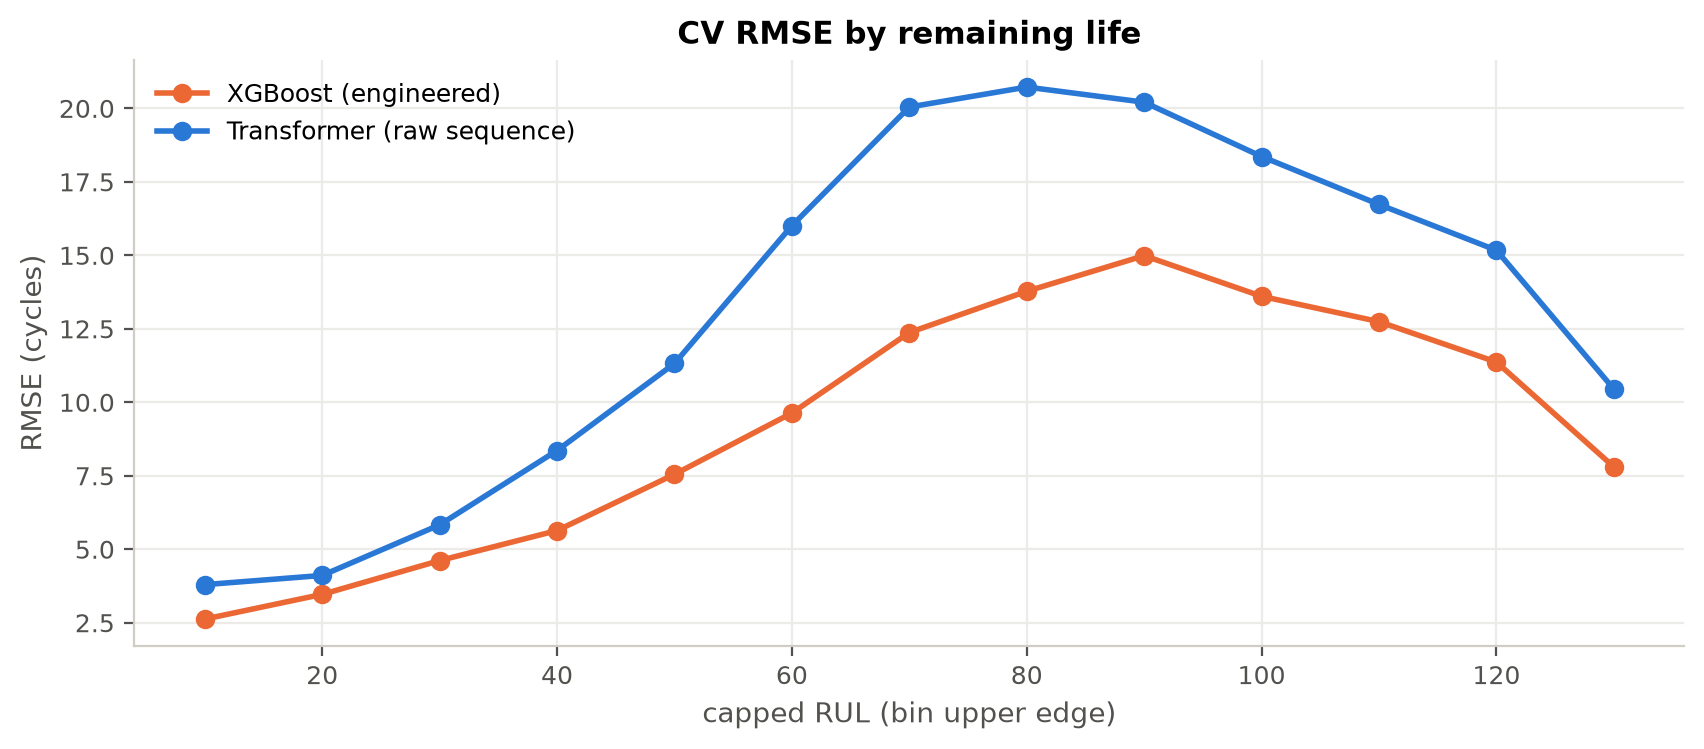
\includegraphics[width=\columnwidth]{07_error_by_rul.png}
  \caption{CV RMSE by remaining life: the sequence model's gap to XGBoost is largest at the onset of degradation.}
  \label{fig:bins}
\end{figure}
